\documentclass[9pt, conference, a4paper, compsocconf]{IEEEtran}
\usepackage{amsmath,amsxtra,amssymb,amsthm,latexsym,amscd,amsfonts}
\usepackage[utf8]{vietnam}
\usepackage[top=2.7cm, bottom = 5.4cm, left=2.72cm, right = 2.85cm]{geometry}
\headsep = 0.7cm
\headheight = 1.0cm 
\footskip = 1.0cm
\voffset = -0.74 cm 
%%%%
\usepackage{balance}

\usepackage{fancyhdr}
\pagestyle{fancy}
\usepackage{cite}
\usepackage{algorithmic}
\usepackage{graphicx}
\usepackage{textcomp}
\usepackage{booktabs}   
\usepackage{tabularx}  
\usepackage{xcolor}
\usepackage{amsmath,amsxtra,amssymb,amsthm,latexsym,amscd,amsfonts}
\usepackage{pgfplots}
\usepackage{multirow}
\usepackage{subcaption}
\pgfplotsset{compat=1.17} 

\usepackage{tikz}
\usetikzlibrary{positioning}  
\usetikzlibrary{arrows.meta}  
\usetikzlibrary{shapes}      
\usetikzlibrary{calc}      
\usetikzlibrary{fit}          
\usepackage[english]{babel} %Figure ... English (có thể bỏ đi nếu bài viết tiếng Việt)
\usepackage{fancyhdr}
\pagestyle{fancy}
%\renewcommand{\chaptermark}[1]{\markboth{\MakeUppercase{#1}}{}}
\renewcommand{\sectionmark}[1]{\markright{\MakeUppercase{#1}}{}}
\renewcommand{\headrulewidth}{0pt}
\ifCLASSINFOpdf
\usepackage[pdftex]{graphicx}
  \DeclareGraphicsExtensions{.pdf,.jpeg,.png,.jpg}
\else
\usepackage[dvips]{graphicx}
  \DeclareGraphicsExtensions{.eps}
\fi
\usepackage{array}

\usepackage{caption}
\captionsetup{
  font={footnotesize}, 
  justification=centering,
  singlelinecheck=false
}
\usepackage[font=footnotesize]{subfig}

\makeatletter
\def\ps@IEEEtitlepagestyle{%
\def\@oddhead{\hfil \small{\textit{Hội thảo khoa học Quốc gia về Trí tuệ nhân tạo 2026 (FJCAI) - Cần Thơ, 27-28/3/2026}\hfil}%
	\def\@evenhead{\hfil\small{\textit{Hội thảo khoa học quốc gia về Trí tuệ nhân tạo 2026 (FJCAI) - Cần Thơ, 27-28/3/2026}\hfil}}%
		\def\@oddfoot{\scriptsize \thepage \hfil }%
		\def\@evenfoot{\scriptsize \hfil \thepage}
	}
}

\def\@maketitle{%
  \newpage
  \null
  \begin{center}%
    {%
      \fontsize{16}{18}\selectfont
      \bfseries \@title \par
    }%
    \vskip 4em%
    {%
    \fontsize{9}{3.5}\selectfont
      
      \begin{tabular}[t]{c}%
        \@author
      \end{tabular}\par
    }%
  \end{center}%
  \par
}

\renewenvironment{abstract}
  {\normalfont
   \if@twocolumn
     \@IEEEabskeysecsize\bfseries\textit{\abstractname}: 
   \else
     \begin{center}\@IEEEabskeysecsize\textbf{\abstractname}\end{center}
     \@IEEEabskeysecsize
     \setlength{\parindent}{0pt}   % ← tắt thụt đầu dòng
     \noindent
   \fi}
  {\par}

\renewenvironment{abstract}
  {\normalfont
   \@IEEEabskeysecsize
   \setlength{\parindent}{0pt}
   \noindent
   \if@twocolumn
     \bfseries\textit{\abstractname}: 
   \else
     \begin{center}\textbf{\abstractname}\end{center}
   \fi}
  {\par}
  
\renewenvironment{IEEEkeywords}
  {\normalfont
   \@IEEEabskeysecsize
   \vspace{0.3em}       
   \setlength{\parindent}{0pt}
   \noindent
   {\bfseries\itshape \IEEEkeywordsname: }\ignorespaces}
  {\par}

\def\IEEEbibitemsep{1.5pt plus .5pt}

\makeatother



\makeatletter
\AtBeginDocument{
  \renewcommand{\abstractname}{Abstract}
}
\renewcommand{\IEEEkeywordsname}{Keywords}
\makeatother



% Anonymous submission switch: \anontrue hides authors, acknowledgment and data links.
\newif\ifanon
\anontrue

% Visible marker for anything not yet measured or confirmed. Search for it before submitting.
\newcommand{\TODO}[1]{\textcolor{red}{[TODO: #1]}}

\begin{document}
\pagenumbering{gobble}
\fontsize{9}{10}
\selectfont

\fancyhead[RE,LO]{\centering{\small{\textit{Hội thảo khoa học Quốc gia về Trí tuệ nhân tạo 2026 (FJCAI) - Cần Thơ, 27-28/3/2026}}}}

\title{LLM-Assisted Relabeling and Aspect-Query Attention for Vietnamese Student Feedback Aspect-Based Sentiment Analysis}

\ifanon
\author{\IEEEauthorblockN{Anonymous Authors}\IEEEauthorblockA{Anonymous Affiliation}}
\else
\author{\IEEEauthorblockN{Đoàn Quang Thắng, Trương Công Lý, Phạm Nguyễn Thanh Nam}
	\IEEEauthorblockA{Vietnam-Korea University of Information and Communication Technology}
	\IEEEauthorblockA{Email: thangdq.22it@vku.udn.vn}
}
\fi

\maketitle

\begin{abstract}
\TODO{Write last, with the measured results.}
\end{abstract}

\begin{IEEEkeywords}
\textbf{\textit{aspect-based sentiment analysis; student feedback; Vietnamese; multi-task learning; LLM-assisted annotation}}
\end{IEEEkeywords}

\IEEEpeerreviewmaketitle

\section{Introduction}
Student feedback helps universities evaluate teaching and training programs, but reading it by hand does not scale. Aspect-based sentiment analysis (ABSA) \cite{pontiki2014semeval,pontiki2016semeval} addresses this by identifying what a comment is about and the sentiment expressed toward each subject.

For Vietnamese, the UIT-VSFC corpus \cite{nguyen2018uitvsfc} offers more than 16,000 human-annotated sentences, with one sentiment and one of four coarse topics per sentence. A single label cannot represent a sentence such as ``the lecturer is enthusiastic, but the lessons are hard to understand''. Sau et al. \cite{sau2021absa} annotated 5,010 sentences with 11 aspect categories and three polarities, but we could not locate a public release of those labels, and the remaining sentences have no aspect-level annotation.

This paper extends aspect-level annotation to the full corpus and studies whether a shared sentence representation limits a multi-task model on the resulting data. Our contributions are:
\begin{itemize}
\item We relabel the full UIT-VSFC corpus (16,175 sentences, 23,910 aspect--sentiment pairs) with an 11-aspect scheme adapted from \cite{sau2021absa}, using an LLM-assisted human-in-the-loop workflow in which reviewers checked every sentence.
\item We provide a multi-seed benchmark from classical models to multi-task Transformers on a fixed split with consistent metrics.
\item We diagnose per-aspect errors of a shared-representation model and evaluate aspect-query attention for aspect detection and sentiment classification through an ablation study. \TODO{Keep only if supported at G4.}
\end{itemize}

\section{Related Work}
\textbf{Student feedback datasets.} UIT-VSFC \cite{nguyen2018uitvsfc} is annotated at sentence level. Sau et al. \cite{sau2021absa} introduced 11 aspect categories on a 5,010-sentence subset and reported a BiLSTM-CNN as their best model. NEU-ESC \cite{mai2025neuesc} is a separate Vietnamese educational corpus for sentiment and topic classification. EduPulse \cite{nguyen2026edupulse} describes an LLM-enhanced opinion mining system for Vietnamese student feedback. Outside Vietnamese, Kastrati et al. \cite{kastrati2020weakly} apply weak supervision to aspect-based analysis of MOOC reviews.

\textbf{Vietnamese ABSA.} Van Thin et al. \cite{vanthin2021corpora} built two sentence-level corpora for Vietnamese ABSA. PhoBERT \cite{nguyen2020phobert} is a widely used pre-trained BERT-style \cite{devlin2019bert} encoder, and BamiBERT \cite{nguyen2026bamibert} is a recent encoder that takes raw text without word segmentation.

\textbf{Representations for aspect categories.} Multi-task learning \cite{caruana1997multitask} shares an encoder across related tasks. Sun et al. \cite{sun2019auxiliary} turn each aspect into an auxiliary sentence. Li et al. \cite{li2020acmimlln} treat words as instances that indicate an aspect category, and Hu et al. \cite{hu2019can} regularize attention across aspects. In multi-label text classification, LSAN \cite{xiao2019lsan} builds a label-specific document representation. We apply a similar idea with one learned query per aspect \cite{vaswani2017attention}.

\textbf{LLM-assisted annotation.} Pangakis and Wolken \cite{pangakis2024keeping} find LLM label quality promising but argue for validation against human labels for each task. Schroeder et al. \cite{schroeder2025human} show that LLM suggestions can change the label distribution produced by human reviewers. Donhauser et al. \cite{donhauser2026annotation} compare annotation sources for German ABSA. For this reason, we report our human review as a correction rate rather than as agreement.

\section{Dataset and Annotation}
\subsection{Label Scheme}
We use the 11 aspect categories of \cite{sau2021absa} (Table~\ref{tab:aspects}) and three polarities. The annotation rules differ from \cite{sau2021absa} in two ways. A suggestion about a specific aspect receives both that aspect and \textit{Suggestion}, and a neutral suggestion is labeled neutral. As a result, the two label sets differ in distribution: \textit{Suggestion} accounts for 12.0\% of our pairs against 2.8\% in \cite{sau2021absa}, and neutral accounts for 14.8\% against 2.1\%. F1 scores on the two datasets are therefore not directly comparable.

\begin{table*}[!t]
\renewcommand{\arraystretch}{1.1}
\caption{\uppercase{Aspect categories and label counts}}
\label{tab:aspects}
\centering
\begin{tabular}{llrrrr}
\toprule
Aspect & Scope & Pos. & Neg. & Neu. & Total \\
\midrule
Teaching Skill & lesson organization and teaching methods & 3,960 & 2,332 & 194 & 6,486 \\
Behavior & lecturer's attitude and communication & 4,943 & 1,294 & 62 & 6,299 \\
Suggestion & students' suggestions and wishes & 474 & 357 & 2,040 & 2,871 \\
Assignment & assignments, their number and types & 446 & 1,011 & 268 & 1,725 \\
Curriculum & curriculum and courses & 196 & 954 & 256 & 1,406 \\
Knowledge & lecturer's subject knowledge & 878 & 288 & 44 & 1,210 \\
Experience & practical experience in lectures & 492 & 341 & 69 & 902 \\
Material Provision & textbooks and learning materials & 268 & 508 & 123 & 899 \\
Teaching Equipment & classrooms, projectors, fans, lights & 37 & 715 & 58 & 810 \\
Grading & grading activities & 78 & 322 & 49 & 449 \\
General & other or general comments & 244 & 239 & 370 & 853 \\
\midrule
Total & & 12,016 & 8,361 & 3,533 & 23,910 \\
\bottomrule
\end{tabular}

\end{table*}

\subsection{Annotation Workflow}
Fig.~\ref{fig:workflow} shows the workflow. For each sentence, gpt-oss-120b received the 11 aspect definitions, the annotation rules and the original UIT-VSFC sentiment and topic as hints, and returned a polarity or ``none'' for each aspect with a confidence score. Human reviewers from our team then checked every sentence, correcting wrong labels or removing the sentence. Because the UIT-VSFC labels served as hints, agreement with them is not independent evidence of quality, and we do not report it as such.

Reviewers had removed 51 sentences during this step, most of them very short. To keep the full corpus and its original split, we restored them: their labels were proposed by a second LLM, Claude, and reviewed by one author, who changed the sentiment of 4 of the 51 sentences.

\begin{figure}[!t]
\centering
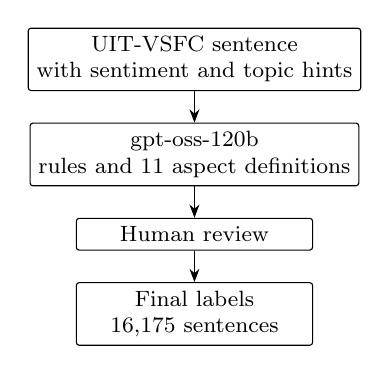
\begin{tikzpicture}[node distance=4mm, box/.style={draw, rounded corners=1pt, align=center, font=\footnotesize, minimum width=30mm, inner sep=3pt}, >=Stealth]
\node[box] (src) {UIT-VSFC sentence\\with sentiment and topic hints};
\node[box, below=of src] (llm) {gpt-oss-120b\\rules and 11 aspect definitions};
\node[box, below=of llm] (rev) {Human review};
\node[box, below=of rev] (final) {Final labels\\16,175 sentences};
\draw[->] (src) -- (llm);
\draw[->] (llm) -- (rev);
\draw[->] (rev) -- (final);
\end{tikzpicture}
\caption{Annotation workflow.}
\label{fig:workflow}
\end{figure}

\subsection{Statistics}
Table~\ref{tab:splits} summarizes the data. We keep the UIT-VSFC train, validation and test split. About 41\% of the sentences hold more than one aspect, so the mean is 1.48 pairs per sentence, against 1.07 in \cite{sau2021absa}.

\begin{table}[!t]
\renewcommand{\arraystretch}{1.1}
\caption{\uppercase{Dataset splits}}
\label{tab:splits}
\centering
\begin{tabular}{lrrrrr}
\toprule
Split & Sentences & Pairs & Pairs/sent. & Multi-aspect & Tokens \\
\midrule
Train & 11,426 & 16,920 & 1.48 & 4,730 & 14.3 \\
Validation & 1,583 & 2,320 & 1.47 & 635 & 13.7 \\
Test & 3,166 & 4,670 & 1.48 & 1,276 & 14.2 \\
All & 16,175 & 23,910 & 1.48 & 6,641 & 14.2 \\
\bottomrule
\end{tabular}

\end{table}

\section{Method}
\subsection{Problem Definition}
Given a sentence $x$, the model predicts a set of pairs $(a, s)$, where $a$ is one of $A = 11$ aspects and $s$ is a polarity. Task A is aspect category detection, a multi-label classification problem \cite{tsoumakas2007multilabel}. Task B is the joint task: a pair is correct only if both the aspect and its polarity are correct.

\subsection{Model}
An encoder turns $x$ into token states $H$ (Fig.~\ref{fig:model}). Each aspect $a$ has a query vector $q_a$. Multi-head cross-attention gives an aspect-specific vector:
\begin{equation}
c_a = \mathrm{MultiHead}(q_a, H, H).
\end{equation}
Both tasks read this vector. Detection uses a separate linear classifier for each aspect, and sentiment uses a shared feed-forward network:
\begin{equation}
p_a = \sigma(w_a^\top c_a + b_a), \quad \hat{s}_a = \mathrm{FFN}([c_a; q_a]).
\end{equation}

\textbf{Query initialization.} Each $q_a$ starts as the mean-pooled encoder output for a short Vietnamese description of the aspect, adapted from \cite{sau2021absa}, and stays trainable. The descriptions were fixed before any error analysis.

\textbf{Loss.} The objective sums binary cross-entropy for detection, with a positive weight for each aspect equal to the square root of its negative-to-positive ratio, clipped to $[1, 20]$, and cross-entropy for sentiment on the aspects present in the sentence, with class weight 2 for neutral and 1 otherwise.

\textbf{Decoding.} Aspect $a$ is predicted when $p_a > \tau$. The threshold $\tau$ is chosen on validation from 0.20 to 0.70 in steps of 0.05 to maximize pair F1. Per-aspect thresholds are reported separately as a secondary analysis.

\begin{figure}[!t]
\centering
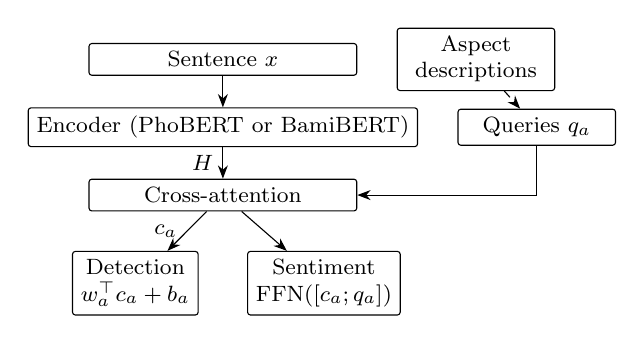
\begin{tikzpicture}[node distance=4mm, box/.style={draw, rounded corners=1pt, align=center, font=\footnotesize, inner sep=3pt}, >=Stealth]
\node[box, minimum width=34mm] (enc) {Encoder (PhoBERT or BamiBERT)};
\node[box, above=of enc, minimum width=34mm] (x) {Sentence $x$};
\node[box, right=5mm of x, minimum width=20mm] (d) {Aspect\\descriptions};
\node[box, below=of enc, minimum width=34mm] (att) {Cross-attention};
\node[box, right=5mm of enc, minimum width=20mm] (q) {Queries $q_a$};
\node[box, below left=5mm and -14mm of att] (det) {Detection\\$w_a^\top c_a + b_a$};
\node[box, below right=5mm and -14mm of att] (sen) {Sentiment\\$\mathrm{FFN}([c_a; q_a])$};
\draw[->] (x) -- (enc);
\draw[->] (enc) -- node[left, font=\footnotesize] {$H$} (att);
\draw[->, dashed] (d) -- (q);
\draw[->] (q) |- (att);
\draw[->] (att) -- node[left, font=\footnotesize] {$c_a$} (det);
\draw[->] (att) -- (sen);
\end{tikzpicture}
\caption{Aspect-query model. The dashed arrow marks initialization only.}
\label{fig:model}
\end{figure}

\section{Experimental Setup}
\textbf{Models.} E0 is TF-IDF with a linear SVM. E1 is a BiLSTM-CNN \cite{hochreiter1997lstm,kim2014cnn} adapted from \cite{sau2021absa}: the architecture matches, while the learning rate, class weights, dropout and preprocessing differ. On PhoBERT, E2 uses mean pooling in both branches, E3 adds query attention to sentiment only, E5 adds it to detection as well, and E4 further initializes the queries from descriptions. E2 and E4 are repeated on BamiBERT. The configuration is fixed across encoders and was not tuned for E4.

\textbf{Training.} Transformer models use AdamW with learning rate $2\times10^{-5}$, weight decay 0.01 and 10\% linear warmup, batch size 16, maximum length 128, dropout 0.3, and at most 8 epochs with patience 2. The checkpoint with the best validation pair F1 is kept. PhoBERT input is word-segmented with underthesea. All models run with seeds 42, 43 and 44; neural models train on an NVIDIA T4.

\textbf{Metrics.} We report micro-F1 for Tasks A and B, as mean and standard deviation over seeds. For each comparison, we compute a 95\% paired bootstrap interval over sentences with 1,000 resamples, recomputing F1 from counts for each seed. We fixed the reporting rule in advance: a difference is called an improvement only if the interval excludes zero and the difference is at least 0.5 F1 points. The test set was scored only after the model and configuration had been locked on validation.

\section{Results and Discussion}
\TODO{Error diagnosis, Table IV (main results), Table V (ablation and encoders), Fig. 3 (per-aspect F1). Fill from results/summary\_test.json after the G3b lock.}

\section{Conclusion}
\TODO{Summary, limitations and future work.} Limitations: no independent double annotation was carried out, so we cannot report inter-annotator agreement; reviewers saw the LLM output and may have been anchored on it \cite{schroeder2025human}; and the original UIT-VSFC labels served as hints during annotation.

\ifanon\else
\section*{Acknowledgment}
The authors thank Dr. Trần Uyên Trang for guidance. \TODO{Confirm the wording and name everyone who helped with labeling.}
\fi

\balance
\bibliographystyle{IEEEtran}
\bibliography{references}

\end{document}
